\PassOptionsToPackage{unicode=true}{hyperref} % options for packages loaded elsewhere
\PassOptionsToPackage{hyphens}{url}
%
\documentclass[]{article}
\usepackage{lmodern}
\usepackage{amssymb,amsmath}
\usepackage{ifxetex,ifluatex}
\usepackage{fixltx2e} % provides \textsubscript
\ifnum 0\ifxetex 1\fi\ifluatex 1\fi=0 % if pdftex
  \usepackage[T1]{fontenc}
  \usepackage[utf8]{inputenc}
  \usepackage{textcomp} % provides euro and other symbols
\else % if luatex or xelatex
  \usepackage{unicode-math}
  \defaultfontfeatures{Ligatures=TeX,Scale=MatchLowercase}
\fi
% use upquote if available, for straight quotes in verbatim environments
\IfFileExists{upquote.sty}{\usepackage{upquote}}{}
% use microtype if available
\IfFileExists{microtype.sty}{%
\usepackage[]{microtype}
\UseMicrotypeSet[protrusion]{basicmath} % disable protrusion for tt fonts
}{}
\IfFileExists{parskip.sty}{%
\usepackage{parskip}
}{% else
\setlength{\parindent}{0pt}
\setlength{\parskip}{6pt plus 2pt minus 1pt}
}
\usepackage{hyperref}
\hypersetup{
            pdfborder={0 0 0},
            breaklinks=true}
\urlstyle{same}  % don't use monospace font for urls
\usepackage[margin=1in]{geometry}
\usepackage{graphicx,grffile}
\makeatletter
\def\maxwidth{\ifdim\Gin@nat@width>\linewidth\linewidth\else\Gin@nat@width\fi}
\def\maxheight{\ifdim\Gin@nat@height>\textheight\textheight\else\Gin@nat@height\fi}
\makeatother
% Scale images if necessary, so that they will not overflow the page
% margins by default, and it is still possible to overwrite the defaults
% using explicit options in \includegraphics[width, height, ...]{}
\setkeys{Gin}{width=\maxwidth,height=\maxheight,keepaspectratio}
\setlength{\emergencystretch}{3em}  % prevent overfull lines
\providecommand{\tightlist}{%
  \setlength{\itemsep}{0pt}\setlength{\parskip}{0pt}}
\setcounter{secnumdepth}{0}
% Redefines (sub)paragraphs to behave more like sections
\ifx\paragraph\undefined\else
\let\oldparagraph\paragraph
\renewcommand{\paragraph}[1]{\oldparagraph{#1}\mbox{}}
\fi
\ifx\subparagraph\undefined\else
\let\oldsubparagraph\subparagraph
\renewcommand{\subparagraph}[1]{\oldsubparagraph{#1}\mbox{}}
\fi

% set default figure placement to htbp
\makeatletter
\def\fps@figure{htbp}
\makeatother

\usepackage{ctex}
\usepackage{xcolor}
\usepackage{fancyhdr}
\pagestyle{fancy}
\cfoot{\thepage}
\usepackage{sectsty}
\definecolor{glaucous}{rgb}{0.38, 0.51, 0.71}
\definecolor{lavenderblush}{rgb}{1.0, 0.94, 0.96}
\usepackage{enumitem}% http://ctan.org/pkg/enumitem
\usepackage[empty]{fullpage}% http://ctan.org/pkg/fullpage
\usepackage{color}% http://ctan.org/pkg/color
\usepackage{hyperref}% http://ctan.org/pkg/hyperref
\usepackage{geometry}
\geometry{a4paper,scale=1}
\usepackage{blindtext}
\usepackage[center]{caption}
\usepackage{subfigure}
\usepackage{float}
\usepackage{graphicx}
\usepackage{booktabs}
\usepackage[justification=centering]{caption}
\usepackage{threeparttable}
\usepackage{longtable}
\usepackage{array}
\usepackage{multirow}
\usepackage{wrapfig}
\usepackage{float}
\usepackage{colortbl}
\usepackage{pdflscape}
\usepackage{tabu}
\usepackage{threeparttable}
\usepackage{threeparttablex}
\usepackage[normalem]{ulem}
\usepackage{makecell}
\usepackage{xcolor}
\linespread{1.0}
\setlength{\parskip}{1em}
\setlength{\footskip}{20pt}
\linespread{1.25}
\textwidth 7in
\textheight 9.95in
\oddsidemargin -.25in
\evensidemargin -.25in
\topmargin -1in
\usepackage{etoolbox}
\makeatletter
\providecommand{\subtitle}[1]{% add subtitle to \maketitle
  \apptocmd{\@title}{\par {\large #1 \par}}{}{}
}
\makeatother
\usepackage{booktabs}
\usepackage{longtable}
\usepackage{array}
\usepackage{multirow}
\usepackage{wrapfig}
\usepackage{float}
\usepackage{colortbl}
\usepackage{pdflscape}
\usepackage{tabu}
\usepackage{threeparttable}
\usepackage{threeparttablex}
\usepackage[normalem]{ulem}
\usepackage{makecell}
\usepackage{xcolor}

\title{\textcolor{glaucous}{\Huge \textbf {新冠早报}}}
\providecommand{\subtitle}[1]{}
\subtitle{\textcolor{glaucous}{\Large 第13期 \space 4月8日}}
\author{}
\date{\vspace{-2.5em}}

\begin{document}
\maketitle

\fontsize{22}{22}
\selectfont
\vspace{-10truemm}

\newcommand{\resheading}[1]{%
  \noindent\fcolorbox{lavenderblush}{lavenderblush}{\makebox[\dimexpr\textwidth-2\fboxsep-2\fboxrule][l]{\textbf{~#1}}}%
}

\pagestyle{fancyplain}
\lhead{
\includegraphics[height=2cm]{./input/logo.png}}
\rhead{
\begin{tabular}{ccc}
\textcolor{gray}{中美健康峰会「智援组」新冠早报组}\\
\\ \\ \\ \\ \\
\end{tabular}}

\renewcommand{\headrulewidth}{0pt}
\setlength{\headheight}{25pt} 
\setlength{\headsep}{-15pt}

%
  \noindent\fcolorbox{lavenderblush}{lavenderblush}{\makebox[\dimexpr\textwidth-2\fboxsep-2\fboxrule][l]{\textbf{~\Huge 每日新闻}}}%

\hypertarget{section}{%
\subsection{\texorpdfstring{\textcolor{glaucous}{\Huge 国际}}{}}\label{section}}

\textbf{\textcolor{glaucous}{有线电视新闻网(CNN)}}:
\textbf{纽约部分县殡仪馆空间不足}

当地时间4月7日,纽约州萨福克县在短时间内新冠死亡病例增多,该县殡仪馆已接近最大容量。目前,纽约州长岛县已计划在农场使用冷藏建筑来帮助储存尸体。

\textbf{\textcolor{glaucous}{纽约时报(NYT)}} :
\textbf{美国财政部正试图扩大对小企业的贷款计划}

当地时间4月7日,美国财政部长史蒂芬·姆努钦表示,为了应对新冠肺炎疫情的冲击,他已向共和党及民主党议员提出再提供2500亿美元,用于扩大一项旨在帮助小型企业从银行获得贷款的计划。

\textbf{\textcolor{glaucous}{英国广播公司(BBC)}} :
\textbf{巴黎禁止白天户外锻炼}

当地时间4月7日,法国累计新冠死亡病例数持续上升并已超过一万例,巴黎当局宣布禁止市民白天在户外运动。新规定从本周三开始实施,于每日早10点至晚7点生效。

\textbf{\textcolor{glaucous}{日本广播协会(NHK)}} :
\textbf{安倍晋三发布紧急事态宣言}

当地时间4月7日下午,由于日本新冠肺炎疫情扩大,日本首相安倍晋三基于新冠肺炎特别措施法发布``紧急事态宣言'',涵盖东京都、神奈川县、大阪县等七个都府区,将持续至5月6日。安倍表示不会实行城市封锁,但呼吁国民配合,避免不必要的外出。

\textbf{\textcolor{glaucous}{华尔街日报(WSJ)}} :
\textbf{印度再次允许出口可能对新冠病毒有效的抗疟疾药物}

当地时间4月7日,应美国总统特朗普要求,印度宣布结束出口羟氯喹的禁令。此前,印度为确保国内药品供应量,于上个月对羟氯喹的出口进行了限制。

\textbf{\textcolor{glaucous}{非洲新闻(Africa News)}} :
\textbf{非洲不会成为新冠疫苗的试验地}

当地时间4月6日,在两位法国科学家宣称新冠病毒疫苗应首先在非洲进行测试后,世界卫生组织总干事谭德赛在新冠肺炎疫情每日发布会中强调,任何地方的任何疫苗接种都将遵循世界公认的方案,非洲不能也不会成为任何疫苗的试验地。

\hypertarget{section-1}{%
\subsection{\texorpdfstring{\textcolor{glaucous}{\Huge 国内}}{}}\label{section-1}}

\textbf{\textcolor{glaucous}{国家卫健委官网}}:
\textbf{中国首次零新增死亡病例}

北京时间4月7日,据国家卫健委报道,4月6日0时至24时,中国全境无新增死亡病例,这是自1月新冠肺炎疫情爆发以来中国国内首次无新增死亡病例。

\textbf{\textcolor{glaucous}{中国民航局官网}}:
\textbf{从26国乘机回国的中国籍旅客需提前填报防疫健康信息}

据北京时间4月7日发布的《关于中国籍旅客乘坐航班回国前填报防疫健康信息的公告》,自4月8日起,从意大利、美国、西班牙等26个国家已购买回国机票的中国籍旅客需要提前填报防疫健康信息。未按要求填报的旅客将无法登机。

\newpage

%
  \noindent\fcolorbox{lavenderblush}{lavenderblush}{\makebox[\dimexpr\textwidth-2\fboxsep-2\fboxrule][l]{\textbf{~\Huge 疫情观察}}}%

\begin{small}
{数据源:约翰霍普金斯大学,The COVID Tracking Project \quad   数据截止至:北京时间3月28日 早4:00}
\end{small}

\hypertarget{section-2}{%
\section{\texorpdfstring{\textcolor{glaucous}{\Huge 一、世界疫情}}{}}\label{section-2}}

\(\quad\)截至北京时间4月8日早6:30,全球累计确诊病例已经达到1,414,738例,累计死亡81,259
例。在180多个出现确诊病例的国家或地区中,有17个国家累计确诊超万人。目前,主要病例集中在亚洲、欧洲及北美洲。发展中国家和地区的疫情发展也不可忽视:拉丁美洲国家的确诊病例数快速增长,非洲国家累计确诊病例已逾一万例。表1显示,法国确诊病例首次超过德国成为欧洲第三,中国确诊病例数已下降至第六位。

\begin{figure}[H]
\caption{世界疫情分布图 (Global Map of Cumulative Confirmed COVID-19 Cases)} %最终文档中希望显示的图片标题
\centering
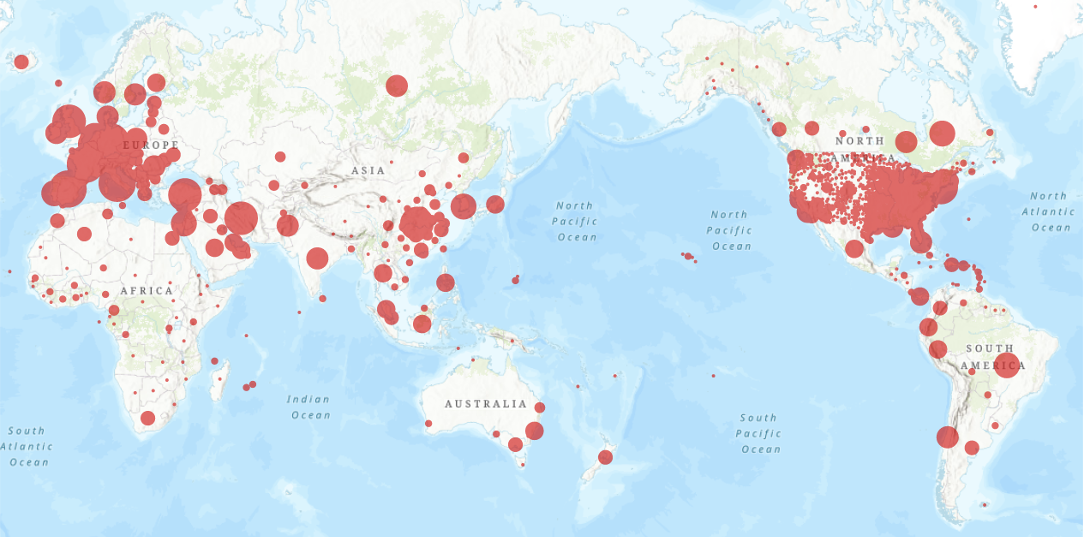
\includegraphics[]{./input/covid1.png} %插入图片,[]中设置图片大小,{}中是图片文件名
\label{} %用于文内引用的标签
\end{figure}

\begin{table}[H]
  \vspace{-7mm}
    \caption{累计确诊前十位国家}
      \vspace{-0.5\baselineskip}
      \centering \begin{table}[H]
\centering
\begin{tabular}{rlrrr}
\toprule
  & 国家(地区) & 累计确诊病例 & 总人口 & 粗发病率\\
\midrule
\rowcolor{gray!6}  1 & 美国 US & 387,547 & 331,002,651 & 117\\
2 & 西班牙 Spain & 140,618 & 46,754,778 & 301\\
\rowcolor{gray!6}  3 & 意大利 Italy & 135,586 & 60,461,826 & 224\\
4 & 法国 France & 110,049 & 65,273,511 & 169\\
\rowcolor{gray!6}  5 & 德国 Germany & 107,591 & 83,783,942 & 128\\
6 & 中国 China & 82,718 & 1,439,323,776 & 6\\
\rowcolor{gray!6}   & 湖北 Hubei & 67,803 & 59,172,000 & 115\\
7 & 伊朗 Iran & 62,589 & 83,992,949 & 75\\
\rowcolor{gray!6}  8 & 英国 United Kingdom & 55,946 & 67,886,011 & 82\\
9 & 土耳其 Turkey & 34,109 & 84,339,067 & 40\\
\rowcolor{gray!6}  10 & 瑞士 Switzerland & 22,253 & 8,654,622 & 257\\
\bottomrule
\end{tabular}
\end{table} \begin{tablenotes}
        \footnotesize
        \item 注:粗发病率定义:累计确诊病例/10万人。计算方式:(累计确诊病例/人口)×10万  %此处加入注释信息
      \end{tablenotes}
    \end{table}

\newpage

\(\quad\)表2和图2显示,美国新增病例数仍居全球首位,已连续八天日新增病例数超过两万人。西班牙与意大利日新增病例数连续下降,意大利昨日新增病例首次跌出日新增国家前五。值得注意的是,法国的日新增病例较昨日翻倍,已突破一万例。同时,土耳其单日确诊病例连续五天增加,提示该地区疫情发展迅速。巴西日新增病例首次进入前十,表明疫情在南美洲有蔓延趋势。

\(\quad\)表3和图3显示,美国的日新增死亡病例再登新高(1,508例),从4月4日至今一直为前十位国家中首位,疫情发展不容乐观。法国的日新增死亡病例数迅速上升,昨日新增死亡病例数仅次于美国,高达1,417例,病死率持续上升,提示该国医疗系统正面临巨大压力。意大利和西班牙的日新增死亡病例数呈下降趋势。

\begin{table}[H]
  \vspace{-7mm}
    \caption{日新增病例前十位国家}
      \vspace{-0.5\baselineskip}
      \centering \begin{table}[H]
\centering
\begin{tabular}{rlr}
\toprule
  & 国家 & 当日新增病例\\
\midrule
\rowcolor{gray!6}  1 & 美国 US & 20,880\\
2 & 法国 France & 11,086\\
\rowcolor{gray!6}  3 & 德国 Germany & 4,217\\
4 & 西班牙 Spain & 3,943\\
\rowcolor{gray!6}  5 & 土耳其 Turkey & 3,892\\
6 & 英国 United Kingdom & 3,667\\
\rowcolor{gray!6}  7 & 意大利 Italy & 3,039\\
8 & 伊朗 Iran & 2,089\\
\rowcolor{gray!6}  9 & 巴西 Brazil & 1,670\\
10 & 比利時 Belgium & 1,380\\
\bottomrule
\end{tabular}
\end{table} \end{table}\begin{table}[H]
  \vspace{-7mm}
    \caption{累计死亡病例前十位国家}
      \vspace{-0.5\baselineskip}
      \centering \begin{table}[H]
\centering
\begin{tabular}{rlrrr}
\toprule
  & 国家 & 累计死亡病例 & 较昨日 & 病死率\\
\midrule
\rowcolor{gray!6}  1 & 意大利 Italy & 17,127 & 604 & 12.6\\
2 & 西班牙 Spain & 13,912 & 571 & 9.9\\
\rowcolor{gray!6}  3 & 美国 US & 12,291 & 1,508 & 3.2\\
4 & 法国 France & 10,343 & 1,417 & 9.4\\
\rowcolor{gray!6}  5 & 英国 United Kingdom & 6,171 & 786 & 11.0\\
6 & 伊朗 Iran & 3,872 & 133 & 6.2\\
\rowcolor{gray!6}  7 & 中国 China & 3,335 & 0 & 4.0\\
8 & 荷兰 Netherlands & 2,108 & 234 & 10.7\\
\rowcolor{gray!6}  9 & 比利時 Belgium & 2,035 & 403 & 9.2\\
10 & 德国 Germany & 2,012 & 202 & 1.9\\
\bottomrule
\end{tabular}
\end{table} \end{table}

\begin{figure}[H]
\caption{日新增确诊病例国家趋势图 \\(中国及其他前五位国家)} %最终文档中希望显示的图片标题
\centering
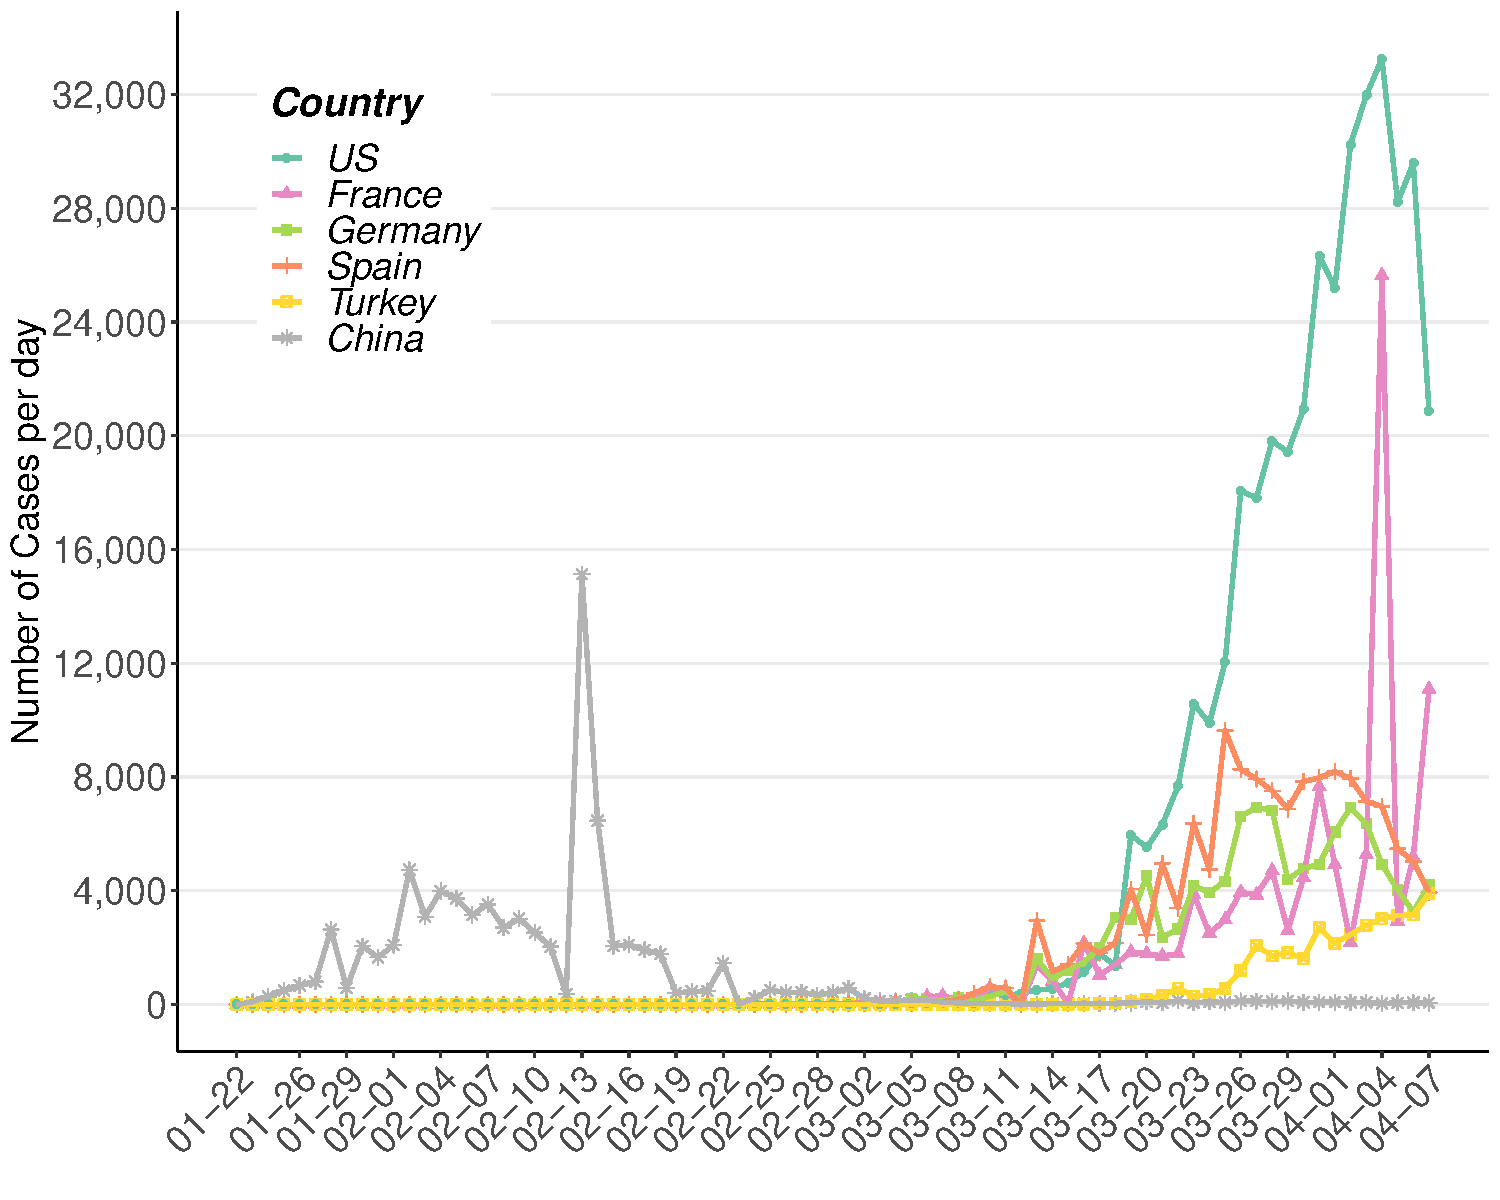
\includegraphics[]{./input/covid2.pdf} 
\label{} %用于文内引用的标签
\end{figure}

\begin{figure}[H]
\caption{日新增死亡病例国家趋势图 \\(中国及其他前五位国家)} %最终文档中希望显示的图片标题
\centering
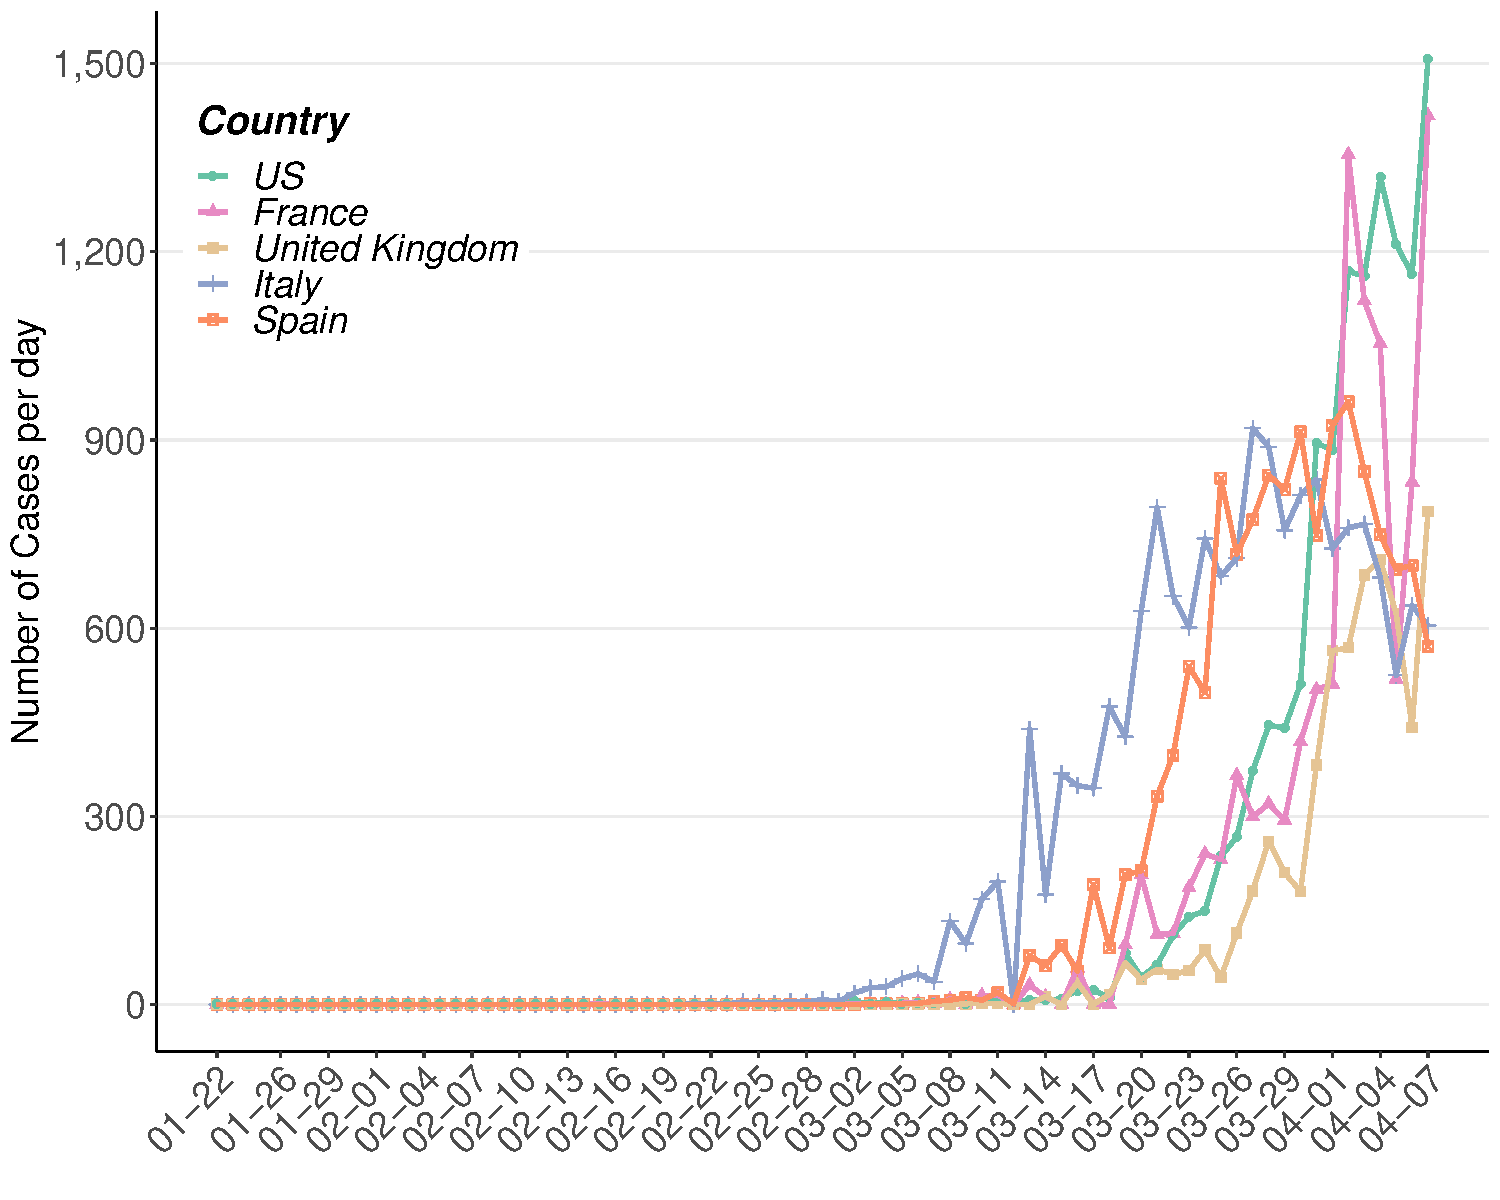
\includegraphics[]{./input/covid3.pdf} 
\label{} %用于文内引用的标签
\end{figure}

\newpage

\hypertarget{section-3}{%
\section{\texorpdfstring{\textcolor{glaucous}{\Huge 二、美国疫情}}{}}\label{section-3}}

\(\quad\)截至北京时间4月8日早6:30,
美国累计确诊病例数已达到387,547例,共 12,291
死亡病例。从州疫情分布图(图4,图5)来看,东西海岸,五大湖及南部地区疫情严重,中部地区疫情呈快速蔓延趋势。

\(\quad\)从表4来看,纽约州(NY)、新泽西州(NJ)和密歇根州(MI)仍为美国疫情最严重的三个州。纽约州粗发病率持续位居全美第一位,高达714/10万人,检测率同为全美最高,达1,748/10万人,而阳性率为全国平均阳性率的2.15倍(41\%),提示该州病人数量巨大,医疗资源持续面临巨大压力。

\(\quad\)值得注意的是,佐治亚州(GA)累计确诊病例首次进入全美前十,取代华盛顿州(WA)。在累计检测人数较少的情况下,佐治亚州的阳性率为26\%,超过美国平均阳性率(19\%),提示该州疫情不容乐观。

\begin{figure}[H] 
\caption{美国本土疫情分布图 (Map of Cumulative Confirmed COVID-19 Cases in Contiguous U.S.)} %最终文档中希望显示的图片标题
\centering
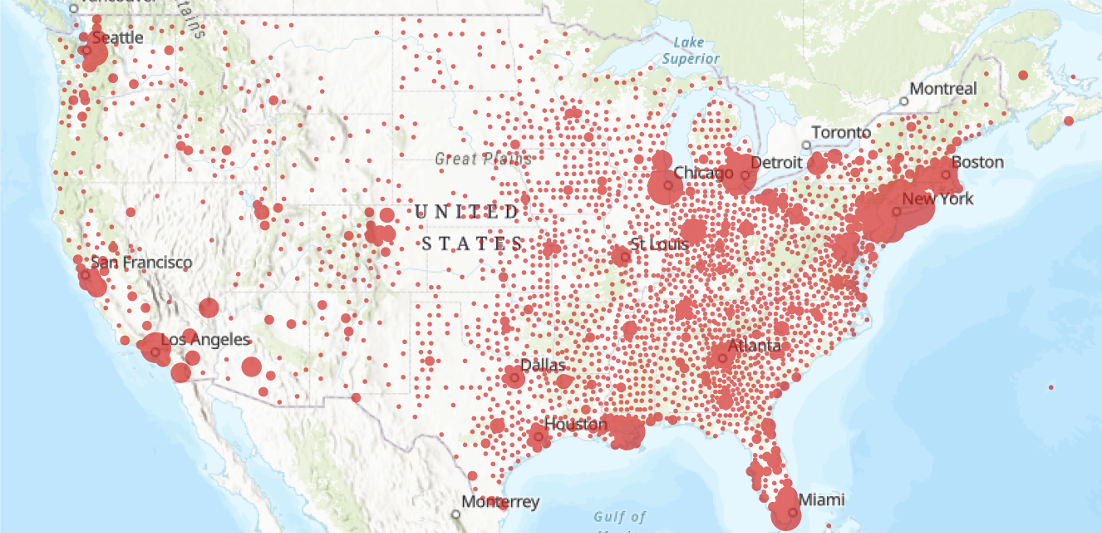
\includegraphics[]{./input/covid4.png} %插入图片,[]中设置图片大小,{}中是图片文件名
\label{} %用于文内引用的标签
\end{figure}

\begin{table}[H]
\vspace{-7mm}
    \caption{美国累计确诊前十位州}
      \vspace{-0.5\baselineskip}
      \centering \begin{table}[H]
\centering
\begin{tabular}{rlrrrrrr}
\toprule
  & 国家/州名 & 累计确诊 & 粗发病率 & 阳性率\% & 累计检测 & 日新增检测 & 检测率\\
\midrule
\rowcolor{gray!6}   & 美国 US & 387,547 & 117 & 19 & 2,054,462 & 137,367 & 621\\
1 & 纽约州 NY & 138,863 & 714 & 41 & 340,058 & 19,247 & 1,748\\
\rowcolor{gray!6}  2 & 新泽西州 NJ & 44,416 & 500 & 47 & 94,974 & 5,942 & 1,069\\
3 & 密歇根州 MI & 17,221 & 172 & 34 & 50,332 & 3,081 & 504\\
\rowcolor{gray!6}  4 & 加利福尼亚州 CA & 16,429 & 42 & 13 & 131,229 & 13,798 & 332\\
5 & 路易斯安那州 LA & 16,284 & 350 & 22 & 74,655 & 5,489 & 1,606\\
\rowcolor{gray!6}  6 & 宾夕法尼亚州 PA & 14,852 & 116 & 16 & 91,278 & 7,424 & 713\\
7 & 佛罗里达州 FL & 14,504 & 68 & 10 & 138,162 & 14,888 & 643\\
\rowcolor{gray!6}  8 & 马萨诸塞州 MA & 13,837 & 199 & 17 & 81,344 & 4,915 & 1,171\\
9 & 伊利诺伊州 IL & 12,266 & 97 & 18 & 68,732 & 5,790 & 542\\
\rowcolor{gray!6}  10 & 乔治亚州 GA & 8,822 & 83 & 26 & 33,713 & 6,299 & 318\\
\bottomrule
\end{tabular}
\end{table} \begin{tablenotes}
    \footnotesize
    \item 注: 检测率定义:累计检测人数/10万人。计算方式:(累计检测人数/人口)*10万
    \end{tablenotes}
    \end{table}

\newpage

\begin{figure}[H]
\caption{美国日新增确诊前五位州趋势图} %最终文档中希望显示的图片标题
\centering
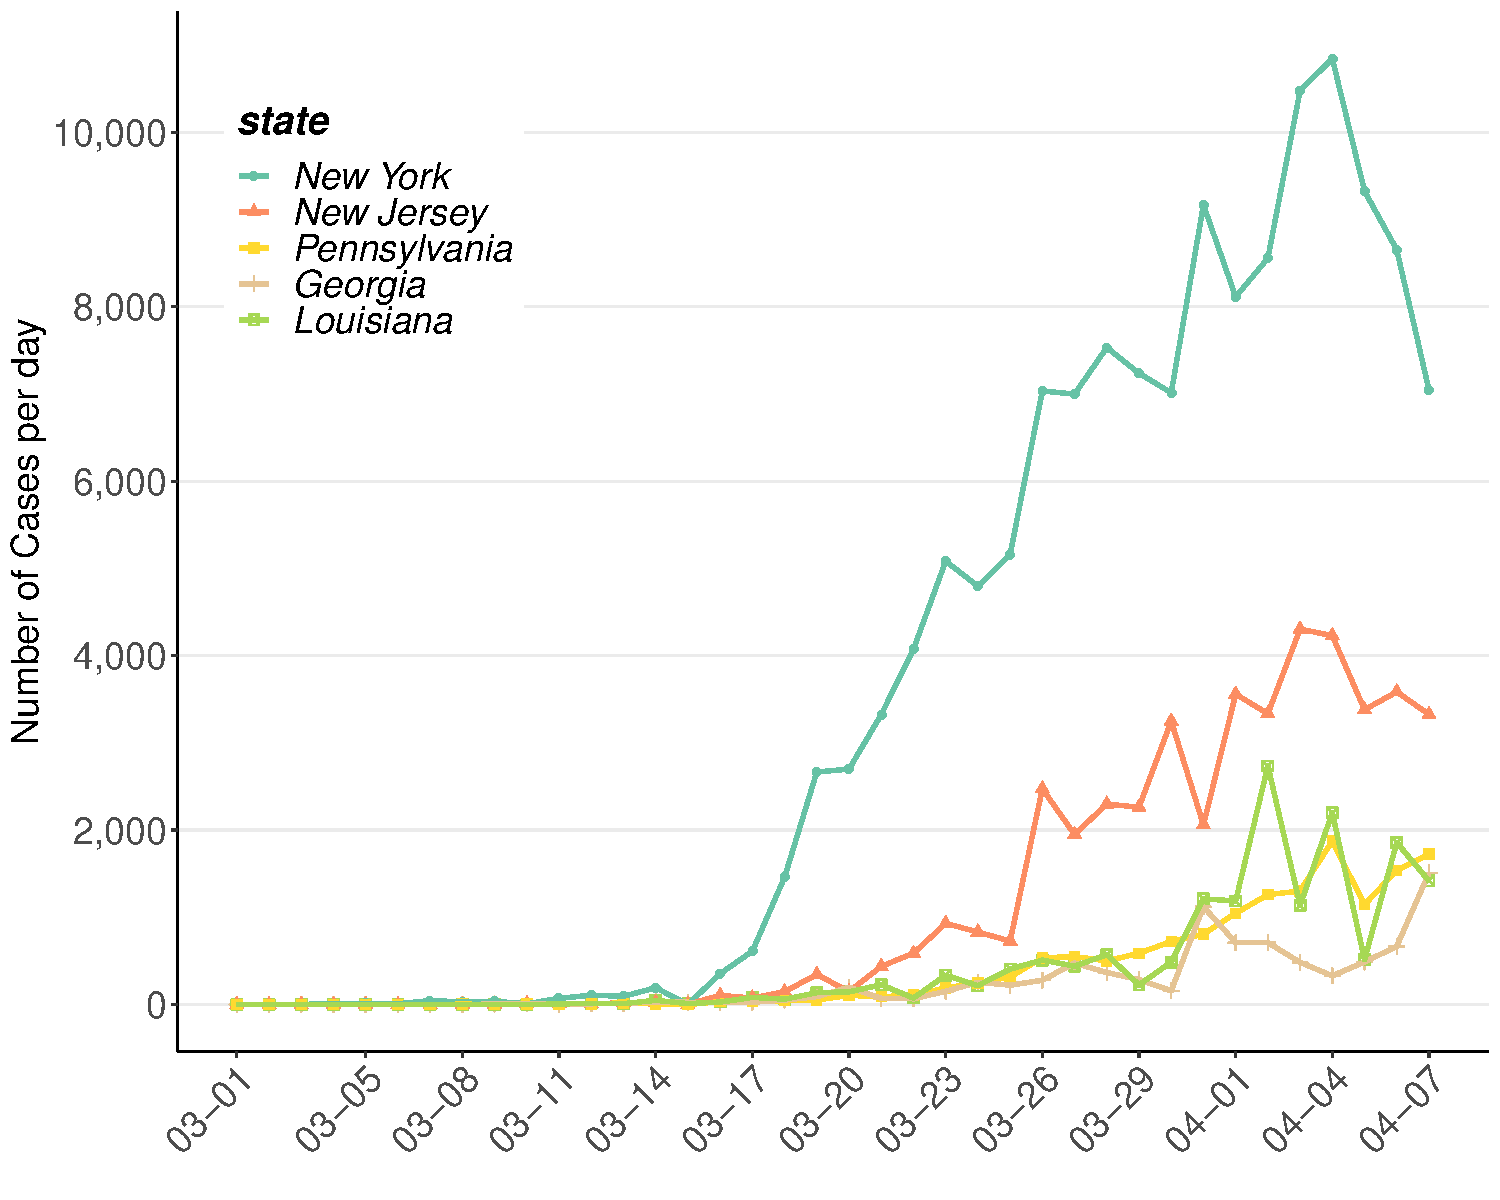
\includegraphics[]{./input/covid5.pdf} 
\label{} %用于文内引用的标签
\end{figure}

\begin{figure}[H]
\caption{美国日新增死亡前五位州趋势图} %最终文档中希望显示的图片标题
\centering
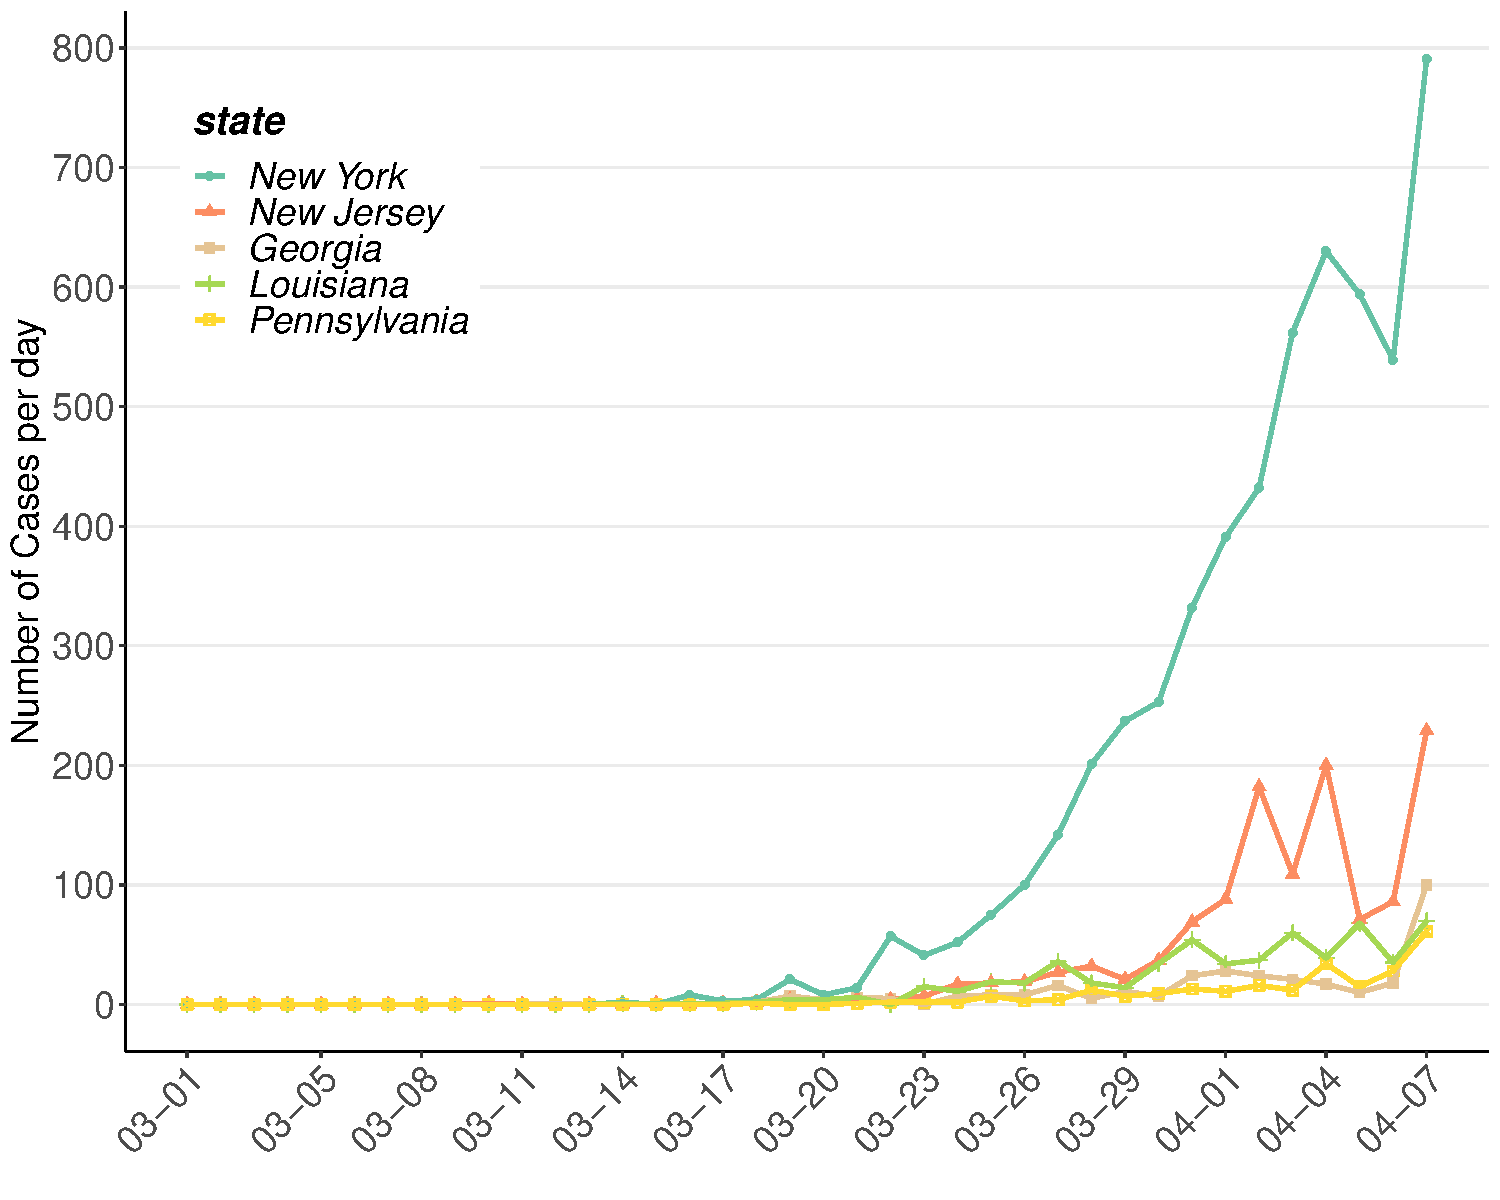
\includegraphics[]{./input/covid6.pdf} 
\label{} %用于文内引用的标签
\end{figure}

\begin{table}[H]
  \vspace{-7mm}
    \caption{美国新增确诊前十位州}
      \vspace{-0.5\baselineskip}
      \centering \begin{table}[H]
\centering
\begin{tabular}{rlrr}
\toprule
  & 国家/州名 & 当日新增 & 全美比率\\
\midrule
\rowcolor{gray!6}   & 美国 US & 20,880 & 100\\
1 & 纽约州 NY & 7,048 & 34\\
\rowcolor{gray!6}  2 & 新泽西州 NJ & 3,326 & 16\\
3 & 宾夕法尼亚州 PA & 1,725 & 8\\
\rowcolor{gray!6}  4 & 乔治亚州 GA & 1,508 & 7\\
5 & 路易斯安那州 LA & 1,417 & 7\\
\rowcolor{gray!6}  6 & 佛罗里达州 FL & 1,180 & 6\\
7 & 印第安纳州 IN & 554 & 3\\
\rowcolor{gray!6}  8 & 弗吉尼亚州 VA & 457 & 2\\
9 & 得克萨斯州 TX & 452 & 2\\
\rowcolor{gray!6}  10 & 加利福尼亚州 CA & 410 & 2\\
\bottomrule
\end{tabular}
\end{table} \end{table}\begin{table}[H]
  \vspace{-7mm}
    \caption{美国累计死亡前十位州}
      \vspace{-0.5\baselineskip}
      \centering \begin{table}[H]
\centering
\begin{tabular}{rlrr}
\toprule
  & 国家/州名 & 累计死亡人数 & 病死率\\
\midrule
\rowcolor{gray!6}   & 美国 US & 12,291 & 3.2\\
1 & 纽约州 NY & 5,489 & 4.0\\
\rowcolor{gray!6}  2 & 新泽西州 NJ & 1,232 & 2.8\\
3 & 密歇根州 MI & 727 & 4.2\\
\rowcolor{gray!6}  4 & 路易斯安那州 LA & 582 & 3.6\\
5 & 加利福尼亚州 CA & 397 & 2.4\\
\rowcolor{gray!6}  6 & 华盛顿州 WA & 388 & 4.6\\
7 & 乔治亚州 GA & 329 & 3.7\\
\rowcolor{gray!6}  8 & 伊利诺伊州 IL & 308 & 2.5\\
9 & 佛罗里达州 FL & 283 & 2.0\\
\rowcolor{gray!6}  10 & 马萨诸塞州 MA & 260 & 1.9\\
\bottomrule
\end{tabular}
\end{table} \end{table}

\(\quad\)从表5新增确诊人数来看,纽约州、新泽西州的新增确诊数仍高居前二,宾夕法尼亚州,佐治亚州,路易斯安那州、和佛罗里达州的日新增确诊病例数均超过1,000人。值得注意的是,佐治亚州的日新增确诊首次进入前五,超1,500例;印第安纳州和佛吉尼亚州日新增确诊也首次进入全美前十。鉴于这些州的人均检测率均低于全美平均值(印第安纳州:427/10万人;佛吉尼亚州:336/10万人),显示这些地区疫情存在恶化的风险。

\(\quad\)从表6来看,美国累计死亡病例已突破一万二千例。纽约州的病死率已上升至4\%,提示纽约州的医疗系统已严重超过负荷。同时,纽约州日新增确诊病例已连续4日下降(图5),可能与居家隔离措施与扩大检测规模有关。值得注意的是,佐治亚州的病死率上升迅速(从4月7日3.1\%到4月8日3.7\%),提示该地区医疗系统正面临巨大挑战。

\newpage

%
  \noindent\fcolorbox{lavenderblush}{lavenderblush}{\makebox[\dimexpr\textwidth-2\fboxsep-2\fboxrule][l]{\textbf{~\Huge 疫情观察}}}%

\hypertarget{section-4}{%
\section{\texorpdfstring{\textcolor{glaucous}{\Huge 全球卫生体系最薄弱国家之一 — 非洲:塞拉利昂}}{}}\label{section-4}}

\(\quad\)据《金融时报》报道,塞拉利昂750万人口,已有6人被确诊新冠肺炎,可塞拉利昂只有一台呼吸机。这台唯一的呼吸机在当地的一家私人医院,当地17家公立医院均无呼吸机。

\(\quad\)造成塞拉利昂防疫形势严峻的原因有很多。主要原因由如下几点:

\begin{enumerate}
\def\labelenumi{\arabic{enumi}.}
\tightlist
\item
  塞拉利昂是世界上最不发达国家之一,经济发展水平落后,医疗资源匮乏。
  1991-2001,该国经历了长达十年之久的内战。在2014年联合国开发计划署发布的人类发展指数排名中,塞拉利昂排名倒数第五。其首都弗里敦的面积只有整个国
  家的1/200,却承受着这个全国1/5人口的压力,且失业率高达70\%。2017年全国注册医生不到200名。
\item
  塞拉利昂的公共卫生体系发展不全面。塞拉利昂曾经是埃博拉病毒的重灾区,尽管在对抗埃博拉之后政府成立了公共卫生应急处理中心,但是由于国内无法量产抗疫物资,依然需要依靠外国援助来解决相关问题。
\item
  新冠疫情已经在非洲大陆快速扩散。截至4月5日,非洲已有51个国家报告出现新冠确诊病例,累计确诊人数8,736人。而两周前,非洲累计确诊人数仅为1,654
  例。在两周之内,非洲确诊人数就增长了4倍。由于防疫能力和资源有限,塞拉利昂无法同时在控制本土病例的同时兼顾严防输入型病例,使疫情防控雪上加霜\(^1\)。
\end{enumerate}

\(\quad\)我国政府长期以来支持非洲公共卫生事业的发展。早在2016年6月,中非就共同签署了《中华人民共和国商务部和非洲联盟委员会关于开展非洲疾病预防控制中心合作谅解备忘录》。2016年塞拉利昂总统欧内斯特·巴伊·科罗马访问中国时特别到访了中国疾控中心,商议中塞公共卫生技术合作相关事宜\(^2\)。

\(\quad\)目前我国国内疫情局势相对稳定,已大规模复工复产,医用防护服、医用防护口罩/面罩、测温仪、呼吸机产能已基本能满足国内需求,企业也正尽力组织扩大出口\(^3\)。在未来一段时间的抗疫物资援助和贸易上,我国相关产业可更多的将目光放在类似塞拉利昂这样的医疗资源和经济基础更加薄弱的国家。

\normalsize 参考文献:

\begin{enumerate}
\def\labelenumi{\arabic{enumi}.}
\item
  南财快评之全球疫情观察:从塞拉利昂看非洲防控
  ~\url{https://k.sina.com.cn/article_1651428902_626ece2602000p2bm.html?from=news\&subch=onews}
\item
  塞拉利昂总统访华,为何首站选择疾控中心?~\url{https://mp.weixin.qq.com/s/lf5e9PfSU7LF-3FiNoi72A}
\item
  工信部:中国呼吸机产能无法满足全球疫情防控需求
  ~\url{https://baijiahao.baidu.com/s?id=1663393284129099919\&wfr=spider\&for=pc}
\end{enumerate}

\centering
\normalsize
\begin{tabular}{ll}

主编:马晶  &  副主编:薛成海\,  仁晖  \\
执行责任编辑:史珂玮 \, 王冠  & 新闻组:张宁\, 张心其 \\
数据分析:杜兆慧  &  案例分析: 史珂玮\\
\multicolumn{2}{l}{可视化组:张立达\, 孙昊\, 唐星鸿\, 齐维为\, 刘逸洋\,张祺珉\,周梓淇}

\end{tabular}

\end{document}
